\chapter{Methods d'optimisation}

Les methodes de optimisation peut se partager en deux sous parties en premier methodes de optimisation avec gradient({\textit{gradient-based}}) et sans gradient ({\textit{gradient-based}}) et dans chaqun de ces categories on peux evoir des problemes de optimisation avec et sans contraintes.
TODO 
\begin{itemize}
    \item Advantages and disadvantages of each of them 
    \item differences 
    \item similarites
\end{itemize}

Algorithme d'optimisation sans contrainte 

Soit $F:\mathbb{R}^d \rightarrow \mathbb{R}$. On suppose qu'il $\exists  x^* \in \mathbb{R}^d$ tel que $F(x^*) = \inf_{x \in \mathbb{R}^d} F(x)$

On cherche a calculer $x^*$

TODO expliquer les methodes dans le diapo 28 de la presentation MIT $16.810_L0_Optimisation$

TODO pas sur de ici si il faut detailler cela ???

Il existe plusieurs classes de methodes:
\begin{itemize}
    \item  Méthodes de descente: consiste à construire une suite minimisante, c'est à dire $(x_k)_{k\in N}$ telle que 
    $$ F(x_{k+1}) \leq F(x_k) $$
    $$x_k \rightarrow x^* $$
    
    \item Méthodes basées sur l'équation d'Euler qui consiste à chercher une solution de l'équation $\nabla F(x) = 0$. Ces méthodes nécessitent donc que $F$ soit dérivable
\end{itemize} 
\section{Heuristic methods}
\section{Methodes base sur des gradients} \label{grad_methods}
Les methodes bases sur les gradients consiste a utiliser le gradient pour se diriger vers ou la fonction decroit et pour en suite trouver un minimum locale. Le deroulement de cela se passe en faisant l'algoritme suivant:
\begin{algorithm}[H]
    \begin{algorithmic}
        \State Initialisation de notre point de depart initale. $x_0 \in \mathbb{R}^d$
        \ForAll {$k$}
            \State Choisir une direction de descente $h_k$ de $F$ au point $x_k$
            \State Choisir un pas $t_k > 0$
            \If{$\nabla F (x_k) = 0$}
                \State \textbf{break} (On arette la boucle car on a trouve notre minimum locale)
            \EndIf
            \State $x_{k+1} = x_k + t_k h_k$
        \EndFor   
    \end{algorithmic}
    \caption{Algorithme de decente generic} % TODO Meilleeur caption
\end{algorithm}


% TODO comment l'exprimer nous meme ou autre alternative
\begin{lemma}[meilleure direction de descente locale] 
Soit $x \in \mathbb{R}^d $ telle que $\nabla F(x) \neq 0$. $h \in \mathbb{R}^d$ est une direction de descente si et seulement si $\langle \nabla F(x), h \rangle < 0$. En particulier, $h_{\nabla} : = -\frac{\nabla F(x)}{\lVert \nabla F(x) \rVert}$ est la meilleure direction de descente.
\end{lemma}

TODO expriquer qqpart la fonction que on choisit peut etre numeroter en $f_1$ et $f_2$ ou $f$ et $g$ 

\subsection{Optimisation sans contrainte}

Soit $F:\mathbb{R}^d \rightarrow \mathbb{R}$. On suppose qu'il $\exists  x^* \in \mathbb{R}^d$ tel que $F(x^*) = \inf_{x \in \mathbb{R}^d} F(x)$

On cherche a calculer $x^*$

% Petit rappell: La heissienne de la fonction $F(\bm{x})$ est note $H_F(\bm x)$ avec $H_F(\bm x)\in \mathcal{M}_d(\mathbb{R})$


\subsection{Methode du gradient a pas constant}
La methode du gradient a pas constant coniste a prendre un point et se deplacer dans la direction contraire du gradient avec un pas consant choisi. La raison la quelle on prends la direction inverse du gradient est que le gradient donne la direction vers ou la fonction croit et nous on veut trouver le minimum. C'ette methode de descente prends un pas constant avec un pas $t_k = \tau > 0$, et une direction de descente $ h_k = - \nabla F(x_k)$. Donc notre formule diteration deviens: 

\[x_{k+1} = x_k - \tau \nabla F(x_k)\]

\begin{table}[H]
    \begin{tabularx}{\linewidth}{>{\parskip1ex}X@{\kern4\tabcolsep}>{\parskip1ex}X}
    \toprule
    \hfil\bfseries Avantages
    &
    \hfil\bfseries Desavantages
    \\\cmidrule(r{3\tabcolsep}){1-1}\cmidrule(l{-\tabcolsep}){2-2}
    %% PROS, seperated by empty line or \par
    Pas nescesaire de connaitre $F$ seulement $\nabla F$ suffit\par
    Pas besoin de iterer pour trouver un pas optimal\par
    &
    %% CONS, seperated by empty line or \par
    Le pas ces' possible que ca ne soit pas optimale\par
    \\\bottomrule
    \end{tabularx}
    \caption{Pros and cons gradient simple}
\end{table}

\begin{figure}[H]
    \centering
    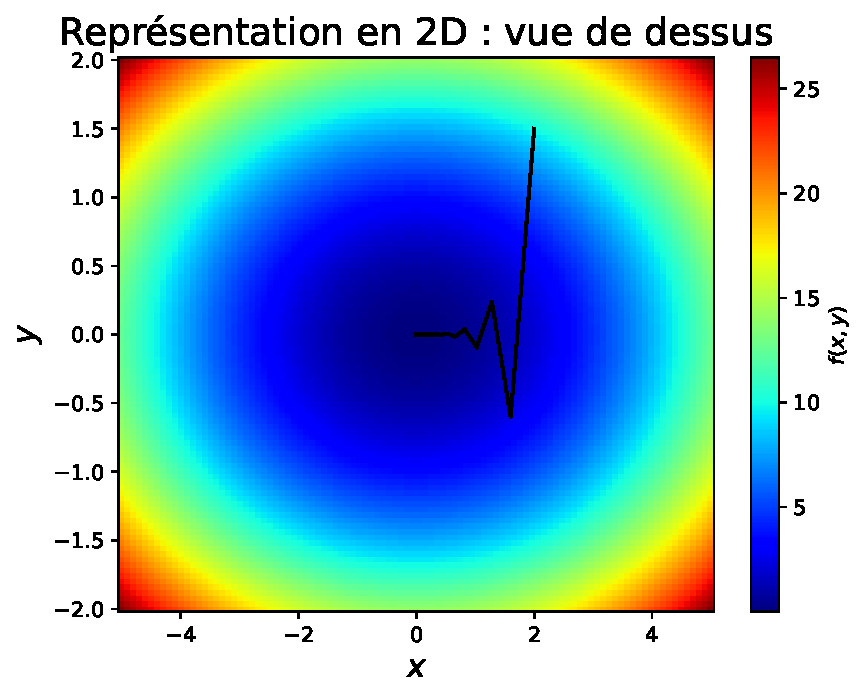
\includegraphics[width = 0.8\textwidth]{TpOpti/grad_pas_cte1.pdf}
    \caption{Figure des iterations avec grad simple en 2D et 3D}
\end{figure}

\begin{figure}[H]
    \centering
    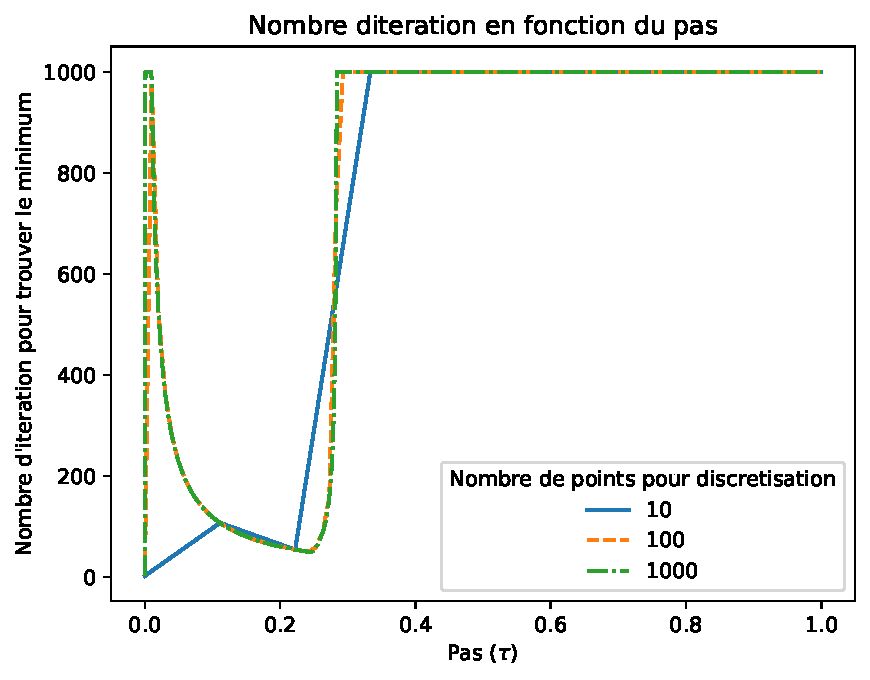
\includegraphics[width = 0.8\textwidth]{TpOpti/discretisation.pdf}
    \caption{Figure du pas optimale droite avec une discretisation elevee gauche discretisation basse}
    \label{fig_optimal_pas_graphe_discretisations}
\end{figure}

\begin{figure}[H]
    \centering
    \includegraphics[width = 0.8\textwidth]{example-image}
    \caption{On choissisant le pas optimale pour avoir le moins de iteration comme vu dans la figure \ref{fig_optimal_pas_graphe_discretisations} le nombre diteration pour chaque point.}
\end{figure}

\subsection{Methode du gradient a pas quasi-optimale}
Dans ces methodes on trouve des pas quasi optimales pour aprocher au minimum avec moins de iterations.
\subsubsection{Regle d'Armijo}
\begin{figure}[H]
    \centering
    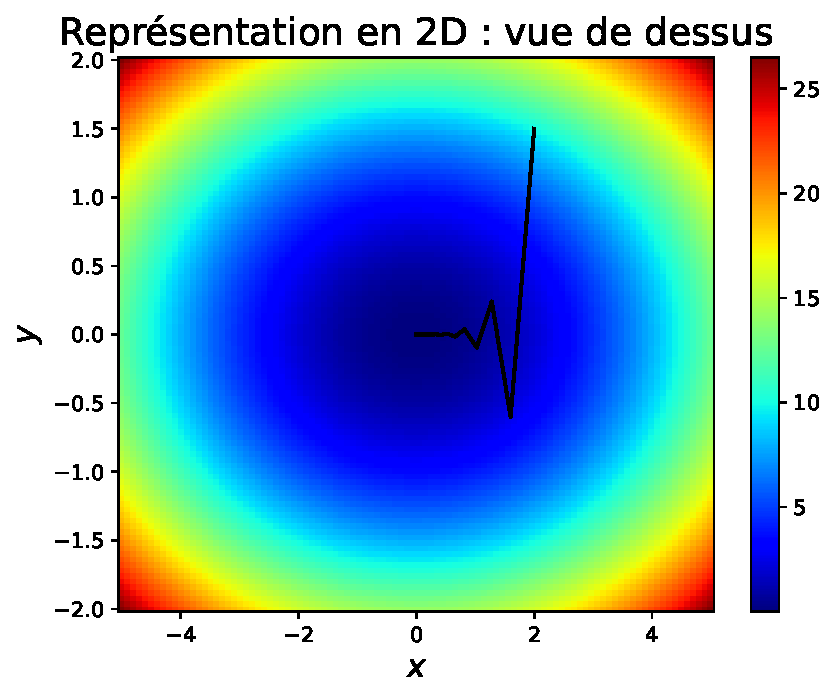
\includegraphics[width = 0.45\textwidth]{TpOpti/Armijo1_0_2.pdf}
    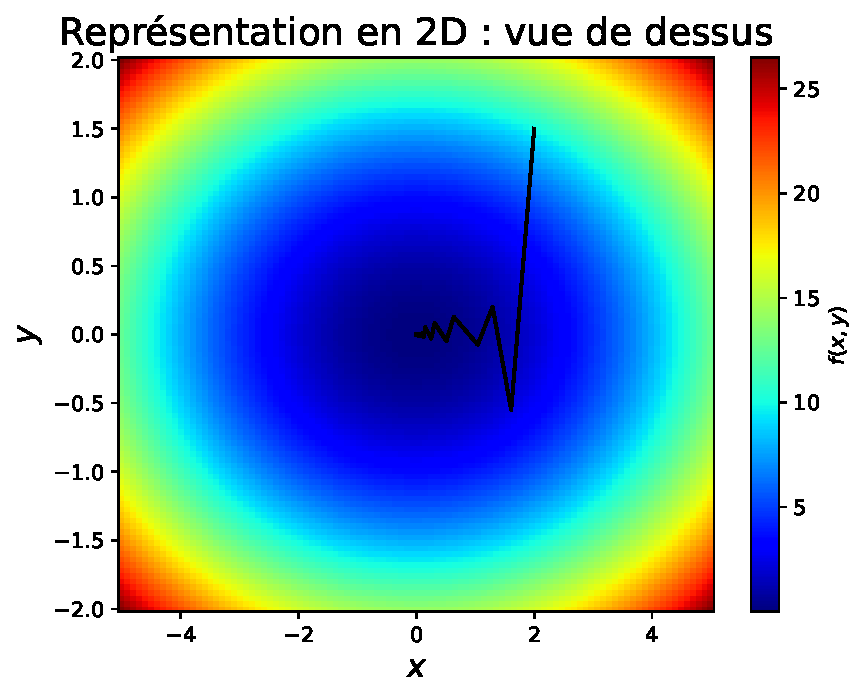
\includegraphics[width = 0.465\textwidth]{TpOpti/Armijo1_100.pdf}
    \caption{TODO add nombre diterations fait}
\end{figure}

\subsubsection{Regle de Wolfe}
\begin{figure}[H]
    \centering
    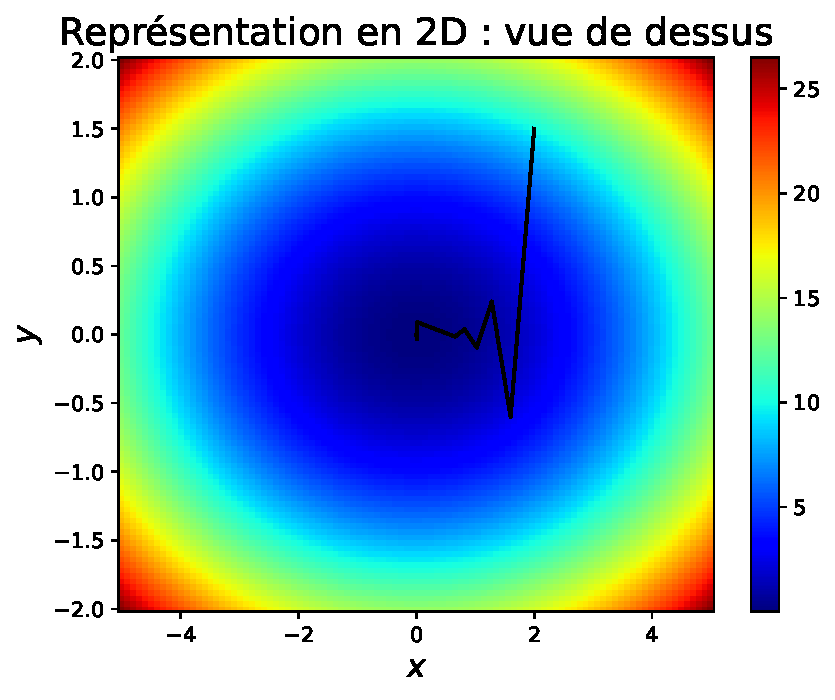
\includegraphics[width = 0.8\textwidth]{TpOpti/Wolfe1.pdf}
    \caption{TODO add nombre diterations fait}
\end{figure}

\subsection{Methode du gradient a pas optimale}
Cette methode essaye de trouver la direction en prennant a la direction orthogonale de la direction precedente. En faisant TODO mettre les formules etc 

On peux voir cette orthogonalite sur la figure TODO cite 3D grad opti

\begin{figure}[H]
    \centering
    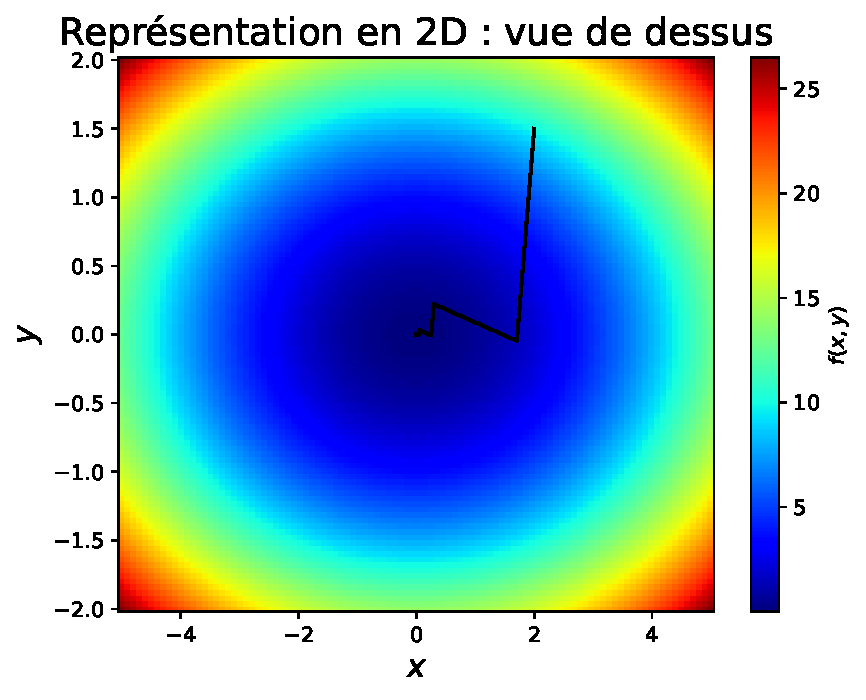
\includegraphics[width = 0.45\textwidth]{TpOpti/grad_opti1.pdf}
    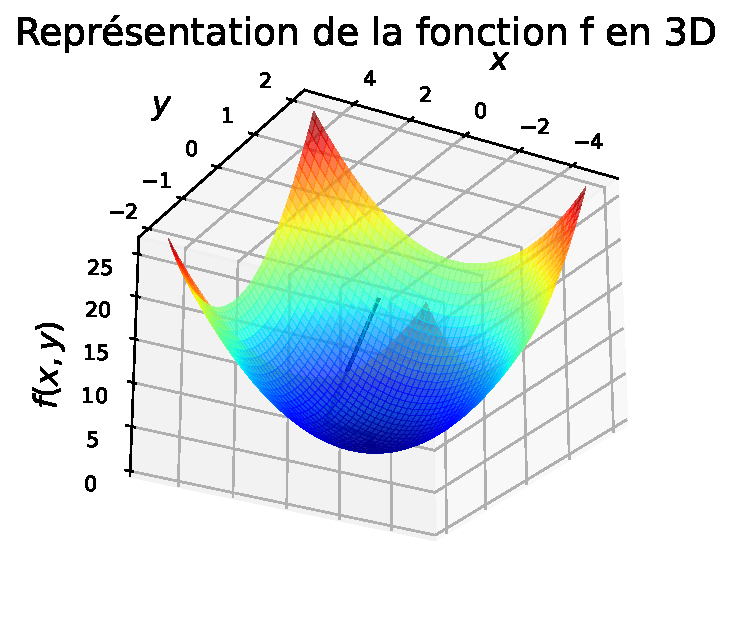
\includegraphics[width = 0.45\textwidth]{TpOpti/grad_opti1_3D.pdf}  
    \caption{TODO add nombre diterations fait}
\end{figure}
\subsection{Adjoint}